\documentclass{beamer}
\usetheme{Madrid}
\beamertemplatenavigationsymbolsempty
\usepackage[utf8]{inputenc}
\usepackage[brazilian]{babel}
\usepackage{listings}
\lstset{
    %frame=tb,
    aboveskip=3mm,
    belowskip=3mm,
    showstringspaces=false,
    basicstyle={\small\ttfamily},
    numbers=none,
    breaklines=true,
    breakatwhitespace=true,
    tabsize=4
}

\setbeamertemplate{footline}{
    \leavevmode
    \hbox{\begin{beamercolorbox}[wd=.175\paperwidth,ht=2.5ex,dp=1.125ex,leftskip=.3cm plus1fill,rightskip=.3cm]{author in head/foot}
        \usebeamerfont{title in head/foot}\insertshorttitle
    \end{beamercolorbox}
    \begin{beamercolorbox}[wd=.825\paperwidth,ht=2.5ex,dp=1.125ex,leftskip=.3cm,rightskip=.3cm plus1fil]{title in head/foot}
        \usebeamerfont{institute in head/foot}\insertinstitute
    \end{beamercolorbox}}
    \vskip0pt
}
\makeatother

\AtBeginSection[]{
    \begin{frame}
    \vfill
    \centering
    \begin{beamercolorbox}[sep=8pt,center,shadow=true,rounded=true]{title}
        \usebeamerfont{title}\insertsectionhead\par%
    \end{beamercolorbox}
    \vfill
    \end{frame}
}

\AtBeginSubsection[]{
    \begin{frame}
    \vfill
    \centering
    \begin{beamercolorbox}[sep=8pt,center,shadow=true,rounded=true]{title}
        \usebeamerfont{title}\insertsubsectionhead\par%
    \end{beamercolorbox}
    \vfill
    \end{frame}
}

\title{RISC-V SiMPLE}
\subtitle{Projeto e Desenvolvimento de processadores RISC-V com a \textit{ISA RV32IMF} usando as microarquiteturas Uniciclo, Multiciclo e \textit{Pipeline} em \textit{FPGA}}
\author{Arthur Matos}
\institute{Universidade de Brasília - UnB}
\date{26 de maio de 2021}

\makeatletter


\begin{document}

\begin{frame}
\titlepage
\end{frame}

\section{Motivação e Objetivos}
    \begin{frame}
        \frametitle{Motivação e Objetivos}
        {}
    \end{frame}

\section{Revisão Teórica}
    \subsection{Arquitetura de computadores}
    \begin{frame}
        \frametitle{Arquitetura de computadores}
        \begin{figure}[H]
        \centering
            \includegraphics[width=.9\textwidth,height=.9\textheight,keepaspectratio]{../images/ABasicComputer.png}
        \end{figure}
    \end{frame}

    \begin{frame}
        \frametitle{RISC vs CISC}
        {Fazer essa parte?} % NOTE: Pensar se faço ou n
    \end{frame}

    \subsection{ISA RISC-V}
    \begin{frame}
        \frametitle{\textit{\textbf{ISA RISC-V}}}
        \begin{figure}[H]
        \centering
            \includegraphics[width=.9\textwidth,height=.9\textheight,keepaspectratio]{../images/riscv_logo.png}
        \end{figure}
    \end{frame}

    \begin{frame}
        \frametitle{Módulo Base}
        {Falar sobre módulo I32/64/128 e E}
    \end{frame}

    \begin{frame}
        \frametitle{Extensões da arquitetura}
        {}
    \end{frame}

    \begin{frame}
        \frametitle{Codificação do tamanho da instrução}
        \begin{figure}[H]
        \centering
            \includegraphics[width=.9\textwidth,height=.9\textheight,keepaspectratio]{../images/RV_InstructionLength.png}
        \end{figure}
    \end{frame}

    \begin{frame}
        \frametitle{Instruções de 32 \textit{bits}}
        \begin{figure}[H]
        \centering
            \includegraphics[width=.9\textwidth,height=.9\textheight,keepaspectratio]{../images/RV_Formats.png}
        \end{figure}
    \end{frame}

    \begin{frame}[fragile]
        \frametitle{Imediatos}
        \begin{lstlisting}
        .text

        ...

        addi    t0, zero, 404
        ...
        \end{lstlisting}
    \end{frame}

    \begin{frame}
        \frametitle{Formação dos imediatos em instruções tipo \textbf{I}}
        \begin{figure}[H]
        \centering
            \includegraphics[width=.9\textwidth,height=.9\textheight,keepaspectratio]{../images/RV_I_Imm.png}
        \end{figure}
    \end{frame}

    \begin{frame}
        \frametitle{Formação dos imediatos em instruções tipo \textbf{S}}
        \begin{figure}[H]
        \centering
            \includegraphics[width=.9\textwidth,height=.9\textheight,keepaspectratio]{../images/RV_S_Imm.png}
        \end{figure}
    \end{frame}

    \begin{frame}
        \frametitle{Formação dos imediatos em instruções tipo \textbf{B}}
        \begin{figure}[H]
        \centering
            \includegraphics[width=.9\textwidth,height=.9\textheight,keepaspectratio]{../images/RV_B_Imm.png}
        \end{figure}
    \end{frame}

    \begin{frame}
        \frametitle{Formação dos imediatos em instruções tipo \textbf{U}}
        \begin{figure}[H]
        \centering
            \includegraphics[width=.9\textwidth,height=.9\textheight,keepaspectratio]{../images/RV_U_Imm.png}
        \end{figure}
    \end{frame}

    \begin{frame}
        \frametitle{Formação dos imediatos em instruções tipo \textbf{J}}
        \begin{figure}[H]
        \centering
            \includegraphics[width=.9\textwidth,height=.9\textheight,keepaspectratio]{../images/RV_J_Imm.png}
        \end{figure}
    \end{frame}

    \begin{frame}
        \frametitle{Programando para a \textit{ISA RISC-V}}
        \begin{figure}[H]
        \centering
            \includegraphics[width=.9\textwidth,height=.9\textheight,keepaspectratio]{../images/rars.png}
            \caption{\textit{IDE RARS}}
        \end{figure}
    \end{frame}

    \subsection{Organização de computadores}
    \begin{frame}
        \frametitle{Organização de computadores}
        \begin{figure}[H]
        \centering
            \includegraphics[width=.9\textwidth,height=.9\textheight,keepaspectratio]{../images/singlecycle_generic.png}
        \end{figure}
    \end{frame}

    \begin{frame}
        \frametitle{Alguns conceitos de microarquiteturas}
        \begin{itemize}
            \item Uniciclo
            \item Multiciclo
            \item \textit{Pipeline}
            \item Superescalar
            \item \textit{Out-of-Order Execution}
        \end{itemize}
    \end{frame}

    \subsection{Representação de \textit{hardware}}
    \begin{frame}
        \frametitle{Representação de \textit{hardware}}
        \begin{itemize}
            \item Programação visual
            \item Linguagens de descrição de \textit{hardware} (\textit{HDL})
            \begin{itemize}
                \item \textit{Verilog}
                \item \textit{VHDL}
            \end{itemize}
            \item Síntese de alto nível (\textit{HLS})
            \begin{itemize}
                \item \textit{C++}
                \item \textit{Matlab}
            \end{itemize}
        \end{itemize}
    \end{frame}

    \subsection{Síntese de \textit{hardware}}
    \begin{frame}
        \frametitle{Sintetizando projetos em \textit{HDL}}
        \begin{figure}[H]
        \centering
            \includegraphics[width=.9\textwidth,height=.9\textheight,keepaspectratio]{../images/quartus/quartus.png}
        \end{figure}
    \end{frame}

    \subsection{\textit{FPGAs}}
    \begin{frame}
        \frametitle{\textit{Field Programmable Logic Arrays}}
        \begin{block}{Arquitetura genérica de uma \textit{FPGA}}
        \begin{figure}[H]
            \begin{subfigure}
            \centering
                \includegraphics[width=.45\textwidth,height=.5\textheight,keepaspectratio]{../images/fpga_architecture_abstraction_-_olin_college.jpg}
            \end{subfigure}
            \begin{subfigure}
            \centering
                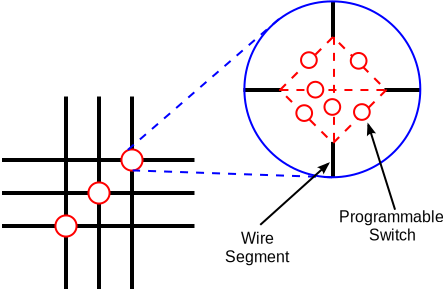
\includegraphics[width=.45\textwidth,height=.5\textheight,keepaspectratio]{../images/switch_box_wikimedia.png}
            \end{subfigure}
        \end{figure}
        \end{block}
    \end{frame}

    \begin{frame}
        \frametitle{\textit{FPGA Altera Cyclone V}}
        \begin{block}{Arquitetura da \textit{FPGA Altera Cyclone V}}
        \begin{figure}[H]
            \begin{subfigure}
            \centering
                \includegraphics[width=.5\textwidth,height=.5\textheight,keepaspectratio]{../images/altera_cyclone_v_soc_architectural_downscale.jpg}
            \end{subfigure}
            \begin{subfigure}
            \centering
                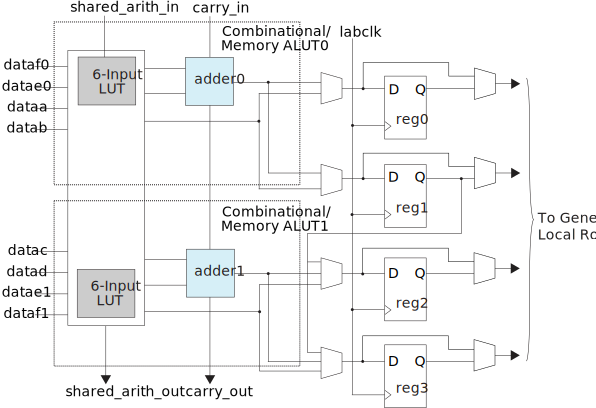
\includegraphics[width=.4\textwidth,height=.5\textheight,keepaspectratio]{../images/intel_alm_high_level.png}
            \end{subfigure}
        \end{figure}
        \end{block}
    \end{frame}

    \subsection{Estado da Arte}
    \begin{frame}
        \frametitle{O Estado da Arte da \textit{ISA RISC-V}}
    \end{frame}

\section{Sistema Proposto}
    \subsection{Organização do projeto}



    \begin{frame}
        \frametitle{}
    \end{frame}

    \begin{frame}
        \frametitle{}
    \end{frame}

    \begin{frame}
        \frametitle{}
    \end{frame}

    \begin{frame}
        \frametitle{}
    \end{frame}


\end{document}

